% 16
\documentclass[output=paper]{LSP/langsci}
\author{Bryan James Gordon}
\title{Information-structural variations in {Siouan} languages}
\abstract{Most previous information-structural\is{information structure} analysis on Siouan languages has been fragmentary and based on incommensurable definitions and frameworks. A \isi{corpus} study drawing on transcribed\is{transcription} and recorded utterances from languages in all major branches of Siouan represents a first step towards generalizable and practical knowledge of the morphosyntactic and \isi{intonation}al indices of information-structural categories in Siouan languages. This study focuses on variations previously noted in the literature -- intonational marking and demarking\is{deaccenting}, \isi{postverbal arguments}, reduction of referring expressions, OSV \isi{word order} and switch-\isi{topic} markers.
% KEYWORDS: [information structure, intonation, postverbal arguments, word order, switch-topic markers, link, recoverability, topic, focus]
}
\ChapterDOI{10.17169/langsci.b94.179}

\maketitle

\begin{document}

\section{Introduction}

	The formal linguistic record offers excellent, comprehensive documentation\is{language documentation} of morphological, syntactic and phonological structures in Siouan languages. The documentary record of those forms’ functions and meanings, however, is hit-and-miss -- fragmented, uncomprehensive, and characterized by individual linguists’ often incommensurable functional analytical frameworks. Most of us documentary linguists\is{language documentation}, in fact, have been trained to seek out, describe and privilege descriptions of context-free levels of semantic meaning, and our work has less to say about the meanings that emerge in and create our linguistic and social contexts, which may well be the most important types of meanings to community-based language-reclamation\is{language revitalization} projects which try to adapt and use our work. The work I present here, while not free of its own analytical framework, attempts to rectify this situation by providing a comprehensive albeit partial description of one area of functional variation in form -- \isi{information structure} -- based on a largely qualitative \isi{corpus} study sampling data from nine Siouan languages.
	
	Most, if not all, previous descriptions of Siouan grammars have had something to say about \isi{information structure}. \citet{Rudin1998}, \citet{Koontz2003} and \citet{Eschenberg2005} provide grammar/\isi{discourse} analyses of specific features of Umoⁿhoⁿ Iye (\ili{Omaha}). \citet[242--260]{Graczyk1991a} and \citet{deReuse1994} describe the functions of \isi{noun incorporation} in \ili{Apsaalooke} (Crow)\footnote{I use autonyms where available for language names, providing the \ili{English} colonial name in parentheses only on first mention. It should not be assumed that the autonyms have the same reference as \ili{English} colonial names. “\ili{Mandan}”, for example, refers to a group of related varieties of which Rų’eta is only one. Where the \ili{English} name is reasonably close in both form and reference to an appropriate autonym, as in the case of ``\ili{Lakota}'', ``\ili{Ho-Chunk}'' or ``\ili{Hidatsa}'', I use the \ili{English} name.} and \ili{Lakota}, respectively. Rood offers analyses of presupposition \citeyearpar{Rood1977} and variation between definite articles \citeyearpar{Rood1985}, also in \ili{Lakota}. \citet{Kaufman2008} offers some information-structural analysis of Taneksą (\ili{Biloxi}). \citet{Wolvengrey1991} describes a switch-\isi{topic} marker (a “focus” marker in his terms) in Rų’eta (\ili{Mandan}). Issues of “oldness”, “emphasis”, “\isi{topic}” and “focus” surface in various formal grammars including Cumberland’s \citeyearpar{Cumberland2005} Nakʰon’i’a (\ili{Assiniboine}) and Boyle’s \citeyearpar{Boyle2007} \ili{Hidatsa} grammar. Ingham’s \citeyearpar{Ingham2003} work is a notably comprehensive discourse-analytical approach to information-structural\is{information structure} variations in \ili{Lakota}. These works, however, generally focus on a single phenomenon, and do not all situate themselves as relevant to a more general field of information-structurally meaningful variation. 
	
	Here I adopt a unifying toolkit which allows us to consider, compare and extend previous findings under a common metalanguage. My hope is not to argue for or against previous analysts’ theoretical or methodological goals, or my own, but to make possible a more coherent and useful conversation about Siouan information-structural\is{information structure} variations for a variety of audiences, including but not limited to theoretical linguists and community-based language-reclamation\is{language revitalization} programs.

\section{Method}

For this study I coded interlinear text from nine languages, and audio data from four, a \isi{corpus} comprising the majority of text and audio available to me at the time of study in 2009. These languages span the four branches of the Siouan language family, including all three subbranches of the large \ili{Mississippi Valley Siouan} subfamily: Rų’eta\il{Mandan}; the \ili{Southeastern Siouan} language Taneksą\il{Biloxi}; the \ili{Missouri Valley Siouan} languages \ili{Hidatsa} and \ili{Apsaalooke}; and the \ili{Mississippi Valley Siouan} languages Nakʰon’i’a\il{Assiniboine}, \ili{Lakota}, \il{Omaha}Umoⁿhoⁿ Iye and \il{Ponca}Paⁿka Iye (Omaha and Ponca), \ili{Ho-Chunk}, and Baxoje Ich\^{}e  and Jiwere Ich\^{}e  (\ili{Ioway} and \ili{Otoe}). Of these I was able to access audio data in \ili{Hidatsa}, Umoⁿhoⁿ Iye, Baxoje Ich\^{}e and Ho-Chunk. My sample, although representative of genetic diversity within the Siouan family, is not balanced across considerations of genre, time period or other sociolinguistic factors. These sources and the speakers who produced them are listed, with an utterance or page count, under “Primary resources” before the references at the end of the chapter. I coded each primary resource for formal variation (\isi{intonation}al, segmental and morphosyntactic criteria summarized in \sectref{intonationcoding}--\sectref{variantselection}) and information-structural\is{information structure} function (criteria summarized in \sectref{informationcoding}). Some of these resources I coded in their entirety; in others (e.g. \citealt{Dorsey1890}) I simply sampled a few works, attempting to capture multiple genres. I also drew many examples for this paper from secondary resources, and they are cited as such when they occur. 

\subsection{Information-structural\is{information structure} coding procedure}\label{informationcoding}

The following is a condensed version of my coding criteria. My criteria are drawn with some modification from the \isi{Givenness Hierarchy} \citep{Gundeletal1993} and Ward \& Birner’s \citeyearpar{WardBirner2001} framework, with attention towards commensurability with other frameworks. Because commensurability is one of my objectives, I do not use the terms ``given,'' ``old,'' ``\isi{topic}'' or ``focus'' without specifying modifiers and definitions. I am the sole coder, so I have no intercoder reliability measure for these criteria, but it may be noted that I was applying Gundel’s criteria in the Minnesota Cognitive Status Research Group\footnote{The Minnesota Cognitive Status Research Group was funded by a National Science Foundation grant, \textit{A cross-linguistic study of reference and cognitive status} (BCS0519890, PI Jeanette Gundel).} at the time this study was conceived, and that we achieved 85\% intercoder reliability. All errors and misapplications are my own.

\ea\label{codingcriteria}
\ea{Code a form as a \textsc{link} if its referent stands in a poset relation with a salient or inferrable alternative. See \citet[121]{WardBirner2001} for examples, and cf. the categories of \textsc{contrast} and \textsc{restriction} in \citet{ErteschikShir2007}. Forms coded as links are \uline{underlined}.}
\ex{Code a form as \textsc{recoverable} if its referent is an \textsc{attention-central} entity or an \textsc{inferrable} \isi{predicate}. These categories are operationalized as in Gundel et al. (\citeyear{Gundeletal1993, Gundeletal2010}), but I replace Gundel’s term \textsc{in focus} with \textsc{attention-central} to avoid confusion with relational focus. A referent is attention-central if its utterer can assume that her audience is consciously attending to it (cf. \textsc{continuing \isi{topic}} in \citealt{ErteschikShir2007}, and \textsc{highly accessible} in \citealt{Ariel1990}). A referent is inferrable if the \isi{discourse} model at time of reference gives ample and recoverable evidence for its validity (if a \isi{predicate}) or existence (if an entity). Such evidence may be logical, narrative, stereotypic or based on general cultural knowledge. Forms coded as recoverable are \textit{italicized}.}
\ex{Code a form as a \textsc{relational \isi{topic}} or \textsc{relational focus} if its referent stands in a directed relation (i.e. a relationship of semantic scope like quantification, or pragmatic/framing scope in the sense of \citealt{Goffman1974}, e.g. stage \isi{topic}s, scene-modifiers, activating \isi{topic}s, extragrammatical mentions, unactivated definites, deixis, “aboutness” and “predication-of”). Relational \isi{topic}s are forms whose referents take scope, and relational foci are forms whose referents are under scope. Forms coded as relational \isi{topic}s are followed by a right angle bracket >, while those coded as relational foci are followed by a left angle bracket <.}\z
\z

Example \REF{codingsummary} diagrammatically represents the coding marks as they are presented in all examples taken from primary sources:

\ea\label{codingsummary}{\uline{link}\hspaceThis{mm} \textit{recoverable}\hspaceThis{mm} relational \isi{topic} >\hspaceThis{mm} relational focus <}\z

\subsection{\is{intonation}Intonation-structural coding procedure}\label{intonationcoding}

Armik \citet{Mirzayan2011} has developed a ToBI coding protocol (cf. \citealt{Pierrehumbert1980}; \citealt{BeckmanPierrehumbert1986}; and \citealt{PierrehumbertHirschberg1990}) for \ili{Lakota}, but at the time of this study no such protocol was available, so I developed one myself. This section principally includes the basic description and justification of the protocol I developed; precise coding criteria have been omitted for length considerations and are available on request. 

I was able to establish consistent criteria for identifying the standard array of prosodic phrase levels -- the \textsc{accent phrase} (AccP), the \textsc{intermediate phrase} (IntP) and the \textsc{\isi{intonation}al phrase} (IP) -- in all four of the sampled languages. Accent phrases in all four languages maximally consist of a low-high-low contour in which either the high point or the high-low fall is accorded greatest prosodic prominence. Such contours are represented in ToBI notation as LH*L, and all four languages have them, although the first L tone in particular is often absent. Intermediate phrases in all four languages consist of one or more accent phrases followed by a phrase accent, either !H or L; and intonational phrases in all four languages consist of one or more intermediate phrases followed by a boundary tone, either !H\% or L\%. The exclamation point before H phrase accents and boundary tones indicates downstep: I found no evidence of upstepped H phrase accents or boundary tones in any of the four languages. 

My protocol was designed to cover four languages (Umoⁿhoⁿ Iye\il{Omaha}, \ili{Ho-Chunk}, Baxoje Ich\^{}e\il{Ioway} and \ili{Hidatsa}) rather than one, and so is shallower and less detailed than Mirzayan’s. The simple apparatus sketched here is designed to capture high-level \isi{intonation}al variations across Siouan languages, and should not be taken as evidence that Siouan intonational structures are simple. Besides \citet{Mirzayan2011} see also \citet{Larson2009} on \il{Omaha}Umoⁿhoⁿ Iye for richer descriptions of intonational variation in particular Siouan languages. 

\subsection{Selection of formal variants of interest}\label{variantselection}

In \isi{information structure} and \isi{intonation}al structure I have begun with high-level, a priori coding categories and attempted to apply them to the entire \isi{corpus}. In deciding which formal (morphosyntactic and segmental as well as intonational) variations to correlate to \isi{information structure}, however, I have made no such attempt. Instead, I have specifically looked at some of the formal variations in previous descriptions of Siouan languages: \isi{postverbal arguments} (\sectref{postverbalarguments}); degrees of reduction of noun phrases or referring expressions, from zero reference to “\isi{determiner drop}” and \isi{noun incorporation} (\sectref{nominalreduction}); OSV \isi{word order} (\sectref{osv}); switch-\isi{topic} markers (\sectref{switchtopic}); and intonational processes of “marking” and “demarking\is{deaccenting}” which surfaced during my ToBI coding (\sectref{intonationalbounding} and \sectref{deaccenting}, respectively).

\section{Findings}\label{findings}

\subsection{Deaccenting\is{deaccenting}}\label{deaccenting}

	I use the term \textsc{deaccenting} to describe \isi{intonation}al variations in which a given word or string of words may be realized either with or without the H* pitch-accent head of an AccP. The variant without the pitch accent is the \textsc{deaccented} variant. This term implies that the accented variant is canonical. \citet[100]{Bolinger1986} makes this explicit: “[A] neutral sentence accents all content words, … and a non-neutral or marked sentence would be one in which one or more words have been deaccented\is{deaccenting}.”
	
Every audio resource I coded has examples of \isi{deaccenting}, and all examples of \isi{deaccenting} signal a recoverable referent. In example \REF{wolfedeaccenting}, \il{Omaha}Umoⁿhoⁿ Iye speaker Clifford Wolfe, Sr.\ia{Wolfe, Sr., Clifford}, deaccents the strings \textit{kʰi égithe} `and so it happened that' and \textit{ahí} `arrived there'. Both are absorbed into the LH*L contour of the AccP headed by \textit{weáhidexti} `truly far':

\renewcommand{\exfont}{\itshape}
\let\eachwordone=\itshape

\ea\label{wolfedeaccenting}
Shkóⁿ-tʰe wasékoⁿ, kʰi égithe weáhidexti ahí.\rmfnm

\glll 	\bjgemph{shkóⁿ-tʰe >}	\bjgemph{wasékoⁿ <}		kʰi 		égithe 		\bjgemph{weáhidexti}		{ahí <}\\
	{\ob L H* L\cb}		{\ob L !H* L\cb\hspaceThis{ }L}		{\ob L}	{}			{H* L}				{\hspaceThis{ahí}\cb\hspaceThis{ }L L\%}\\
	movement-the 		fast 				and 		it.happened.that 	ahead.really	 		arrive.there.\textsc{prox}\\
\footnotetext{Rudin\ia{Rudin, Catherine} field tapes}
\glt `She was moving fast, so it happened that she got pretty far ahead.'
\z

In example \REF{wolfedeaccenting} and in other audio examples, I provide a ToBI line under the information-structural\is{information structure} coding and above the gloss line. Here, AccP’s are represented by square brackets. IntP’s are recognisable by their pitch accents outside square brackets, and the IP by its boundary tone. 

For this example, I also provide a Praat \citep{BoersmaWeenink1992} screenshot, but omit it from subsequent examples due to space considerations. In the screenshot, the blue line is the pitch contour in Hz, and the green line the intensity contour in dB.\footnote{It should further be noted that the blue line, being a computed estimate of pitch, is not sufficient evidence for any ToBI coding criterion, but must be accompanied by impressionistic auditing.} The ToBI line in my Praat annotations is simplified relative to the ToBI line in the examples presented in this paper. Glosses in the Praat annotations are provided at the IntP level, which is a technique I use to simulate the intermediate-level prosodic chunking present in the audio.

\begin{figure}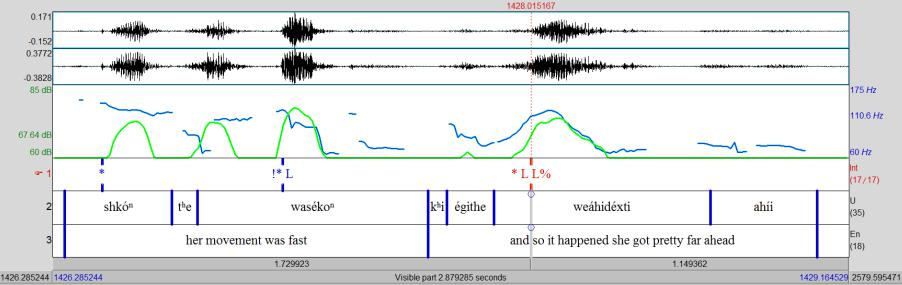
\includegraphics[width=12cm]{figures/Gordon1}\caption{Praat screenshot corresponding to example \REF{wolfedeaccenting}}\label{wolfedeaccentingscreenshot}\end{figure}

In example \REF{wolfedeaccenting}, two sections have been deaccented\is{deaccenting} and absorbed into the L tones that bound an adjacent H* phrase accent. Both have been coded as recoverable: \textit{kʰi égithe} because it is a frequent \isi{discourse} marker that is likely always recoverable in narrative. The \isi{predicate} \textit{ahíi} is inferrable given immediately preceding references to motion, speed and distance.

We may distinguish between “true” \isi{deaccenting}, as in example \REF{wolfedeaccenting}, where the deaccented\is{deaccenting} part of the pitch contour is either flat or very slowly declining, and “weak” \isi{deaccenting}, as in example \REF{wolfeweakdeaccenting}, where Mr. Wolfe\ia{Wolfe, Sr., Clifford} uses a compressed version of the LH*L contour. We are looking at \textit{níkshiⁿga}, whose ToBI line is annotated with (LM*L). This is because the pitch range of this contour is compressed within a range smaller than the pitch range of the L tone in the adjacent AccP, so that it is realized as something more like (LM*L) than a full [LH*L] AccP.

\todo{is the sc at lm* l intended?}
\todo{Check underlining}
\ea\label{wolfeweakdeaccenting}
Hiⁿbéazhi-tʰe égithe, táxti sí-tʰe, thiwágazui níkshiⁿga.\rmfnm\\
\glll	\bjgemph{hiⁿbé-ázhi-tʰe}	{\uline{égithe} >}				\bjgemph{táxti}		\bjgemph{sí-tʰe} 		\bjgemph{thiwágazui}	\bjgemph{níkshiⁿga}\\
	{\ob L H* L}				{\hspaceThis{égithe}\cb\hspaceThis{ }!H}	{\ob L H* L\cb}			{\ob L !H* L\cb}				{\ob L H* L}			{\op \textsc{l m* l}\cp\cb\hspaceThis{ }L L\%}\\
	moccasin-not-that			it-happened-that					deer					foot-that				notice-\textsc{prox}		person\\
\footnotetext{Rudin\ia{Rudin, Catherine} field tapes}
\glt	`The man noticed that she was not wearing shoes, but rather had the feet of a deer.'
\z

\citet[121--123]{Mirzayan2011} presents similar compressed AccP’s in \ili{Lakota}. This phenomenon may suggest a continuous process at work, in which the degree of accenting in AccP’s is continuously gradient. Such a process would challenge the usefulness of a discrete annotation system like ToBI for capturing \isi{deaccenting} phenomena in Siouan languages. If this scale from “true” to “weak” \isi{deaccenting} corresponds to variation in information-structural\is{information structure} function, however, my coding criteria have not captured it. Instead, all types of \isi{deaccenting} I have described signal recoverability of referents. This finding is entirely dependent on my methodology, however, and the area of gradient \isi{deaccenting} and potential information-structural corollaries needs to be investigated further.

In short, all the audio resources I coded display deaccented\is{deaccenting} forms, and all such forms have recoverable referents.

\subsection{Postverbal arguments}\label{postverbalarguments}

Since all Siouan languages canonically position verbs after their arguments, the syntactic status of \isi{postverbal arguments} is controversial. All Siouan languages at very least permit postsentential referring expressions to clarify one or more verbal arguments, but grammarians have varied in accepting \isi{postverbal arguments} as elements of the same sentence (cf. \citealt{Rudin1998}; \citealt{Mithun1999}; \citealt[76]{Ingham2003}; \citealt[421]{Cumberland2005}; \citealt[292--293]{Boyle2007}; \citealt{Gordon2008}). My attention to \isi{deaccenting} phenomena in this study may shed light on this question and enabling language workers to distinguish between those \isi{postverbal arguments} which are clearly “outside” the sentences and those which are more likely “inside”.

Accented \isi{postverbal arguments} (those which are pronounced with the [LH*L] contour of an AccP) typically have nonrecoverable referents. Instead, they clarify uncertain information, providing new information about both entities and \isi{predicate}s. (See \citealt[103]{Graczyk1991a} for a relevant discussion on \ili{Apsaalooke} afterthought.) Accented \isi{postverbal arguments} are usually separated from the verb not only by an AccP boundary but by a prosodic break (i.e. an IntP phrase accent or IP boundary tone). In example \REF{thigrepiraye}, Baxoje Ich\^{}e\il{Ioway} speaker ThigréPi\ia{ThigréPi} concludes an IntP on \bjgemph{ráye uⁿk\^{}úⁿñe\^{}suⁿ} `they gave me a name', as seen in the L phrase accent, here evidenced by early and sustained low pitch. Then he adds another IntP in pronouncing the postverbal argument \bjgemph{Baxóje ráye} `a Baxoje name':\footnote{Square brackets in the ToBI line here refer to IntP boundaries rather than AccP boundaries as previously.}

\ea\label{thigrepiraye}
Woxáñi migragáñi\^{}suⁿ, ráye, ráye uⁿk\^{}úⁿñe\^{}suⁿ, Baxóje ráye.\rmfnm\\
\glll	\bjgemph{woxáñi} 	\bjgemph{migragáñi\^{}suⁿ <}		\bjgemph{ráye <}	ráye		\bjgemph{uⁿk\^{}úⁿñe\^{}suⁿ <}	\bjgemph{Baxóje <}		ráye\\
	{\ob L H* L}		{\hspaceThis{migragáñi\^{}s}L\cb}	{\ob L H* L L\cb}	{\ob L H* L}	{\hspaceThis{uⁿk\^{}úⁿñe}L\cb}	{\ob L !H* L} 		{L\cb\hspaceThis{ }L\%}\\
	cherished	me.their.named.now	name		name	me.give.\textsc{pl}.now	\ili{Ioway}			name\\
\footnotetext{\iai{ThigréPi} in \citet{GoodTracks2004b}}

\glt	`They named me as a cherished one, a name, they gave me a name, a Baxoje name.'
\z

Deaccented\is{deaccenting} \isi{postverbal arguments}, in contrast -- like \bjgemph{níkshiⁿga} in example \REF{wolfeweakdeaccenting} -- are not separated by prosodic breaks, and signal recoverable referents. Example \REF{wilkinsonpostverbal} is a useful model of the relationship between \isi{postverbal arguments} and recoverability in general. \ili{Hidatsa} speaker Helen Wilkinson\ia{Wilkinson, Helen} says \bjgemph{kúahe} `this' first in preverbal position when it is not recoverable, and then in postverbal position when in the second sentence (with the form \bjgemph{kúac} it is recoverable):

\ea\label{wilkinsonpostverbal}
Kúahe aku-iháaraci. Maapúkšaruxpáaka wáahaapʰaak ráahaa’he ita-arukiwé’ kúac.\rmfnm\\
\gll	\bjgemph{kúahe >}	\bjgemph{aku-iháaraci <}	\bjgemph{\uline{Maapúkšaruxpáaka}} 	\bjgemph{\uline{wáahaapʰaak}} 	\bjgemph{\uline{ráahaa’he}}			\bjgemph{\uline{ita-arukiwé’} <}		kúac\\
	Here.this 		different.sorta		Snake.People 					raid 						go.\textsc{caus}.that 				their.story.tell 					here.this\\
\footnotetext{\citet[18: 1]{ParksJonesHollow1978}}
\glt	`This is a different story [from the story of the Bird Woman]. This is the story of the Shoshone raid.'
\z

There are some examples of multiple \isi{postverbal arguments}. In example \REF{multiplepostverbal}, I present two. In example \REF{wilkinsonmultiplepostverbal}, Helen Wilkinson\ia{Wilkinson, Helen} first gives us the recoverable postverbal argument \bjgemph{maa-iháa’š} `the enemy' before then further specifying \bjgemph{Waapúk\-šaruxpáaka’š} `the Snake People'. Although the two phrases share the same entity referent, the function of \bjgemph{Waapúkšaruxpáaka’š} is to supply a \isi{predicate} which is not inferrable at this point in the \isi{discourse} model, so \bjgemph{Waapúkšaruxpáaka’š} is coded nonrecoverable (one of the few unseparated by commas which I coded nonrecoverable). In example \REF{baxojemultiplepostverbal}, however, the telling of the Baxoje legend of Béñeiŋe recorded by Gordon \citet{Marsh1936} displays two \isi{postverbal arguments}. Here the two are not coreferent, nor are they in the same argument relation to the verb, and they are both recoverable. 

\ea\label{multiplepostverbal}
\ea\label{wilkinsonmultiplepostverbal}
Hii šee awá ihtúutiru ú’šiak káawarec maa-iháa’š Waapúkšaruxpáaka’š.\rmfnm\\
\gll	hii 		\bjgemph{šée} 		\bjgemph{awá >}		\bjgemph{ihtúutiru} 			\bjgemph{ú’šiak} 		\bjgemph{káawarec <}	maa-iháa’š 				\bjgemph{Waapúkšaruxpáaka’š <}\\
	and 		that	 		ground 			hill.base.at	 			arrive.\textsc{ss} 		be.there.\textsc{pl.ne}	enemy.\textsc{pl.def}.the 		Snake.People.\textsc{pl.def}.the\\
\footnotetext{\citet[22: 26]{ParksJonesHollow1978}}
\glt	`And the enemy, the Shoshone, were on that ground, having gotten to the base of the hill.'
\ex\label{baxojemultiplepostverbal}
Nahésge, igwáhuŋa súŋe Béñeiŋe.\rmfnm\\
\gll	\bjgemph{nahésge >}	\bjgemph{igwáhuŋa <}	súŋe 		Béñeiŋe\\
	be.if 			his.know 			horse 		Béñeiŋe\\
\footnotetext{\citet{Marsh1936}}
\glt	`And so the horse\textsubscript{i} recognized his\textsubscript{i} [owner] Béñeiŋe.'
\z\z

Without audio we can’t be sure whether the apparent double \isi{postverbal arguments} are really all part of the same utterance, but it makes sense to speculate that, of the two, Ms. Wilkinson’s example \REF{wilkinsonmultiplepostverbal} is more likely to involve a major prosodic break than the Baxoje Ich\^{}e\il{Ioway} example \REF{baxojemultiplepostverbal}.

In written transcripts\is{transcription} for which no audio is available, I found the transcriber’s comma a somewhat useful index of prosody -- and recoverability. Many of the \isi{postverbal arguments} I coded -- like Ms. Wilkinson’s\ia{Wilkinson, Helen} in example \REF{wilkinsonpostverbal} -- were not separated by commas from preceding material. Although transcriber’s commas may somewhat reliably correlate with IntP or IP boundaries as annotated in ToBI, we cannot be too sure of how strong this correlation is. Still, nearly all of the \isi{postverbal arguments} not separated by commas had recoverable referents. Presence of a comma, on the other hand, does not seem to reliably predict recoverability of the referent.

Not all languages (or speakers) are alike with respect to the frequency of \isi{postverbal arguments}. I found many examples of postverbal reference to recoverable entities in Taneksą\il{Biloxi}, Rų’eta\il{Mandan}, \ili{Hidatsa}, and \il{Omaha}Umoⁿhoⁿ Iye and \il{Ponca}Paⁿka Iye texts, and very low rates in \ili{Ho-Chunk} and \ili{Apsaalooke} texts -- but still nearly all of the \isi{postverbal arguments} in the \ili{Ho-Chunk} and \ili{Apsaalooke} texts I coded had recoverable referents. All the languages I looked at allow at least some use of \isi{postverbal arguments} to refer to recoverable entities. In some languages, like \il{Omaha}Umoⁿhoⁿ Iye and \il{Ponca}Paⁿka Iye, this use may be (or have been) obligatory. In \citet{Gordon2008}, I sampled 51 continuing \isi{topic}s in \il{Omaha}Umoⁿhoⁿ Iye and \il{Ponca}Paⁿka Iye and found 42 of them were referred to postverbally. Of the 9 preverbal, most were within repeated collocations. This suggests that in some languages recoverable referents not only \bjgemph{can} be referred to postverbally, but \bjgemph{must} in most contexts.

To summarize, all the languages in this study make use of \isi{postverbal arguments}, although they vary in frequency. Even without audio data to distinguish between deaccented\is{deaccenting} and accented \isi{postverbal arguments}, the strong tendency is observable for \isi{postverbal arguments} to refer to recoverable entities. The index of the transcriber’s\is{transcription} comma may serve as circumstantial evidence. Its absence indirectly indexes recoverability of postverbal referents while also directly, if weakly, indexing \isi{deaccenting}. Forms with nonrecoverable referents are often found after commas, on the other hand. Where audio data is available, the case is clearer: deaccented \isi{postverbal arguments}, like other deaccented material, have recoverable referents, and are intrasentential (part of the same sentence as the verb they follow) by \isi{intonation}al if not syntactic criteria.

\subsection{Reduced nominal referring expressions}\label{nominalreduction}

\subsubsection{Determiner drop\is{determiner drop} in languages with two indefinite articles}\label{droptwoindef}

Of the languages represented in this study, four -- \ili{Lakota}, Nakʰon’i’a\il{Assiniboine}, \ili{Apsaalooke} and \ili{Ho-Chunk} -- have two indefinite articles, one specific and one nonspecific. The texts I coded in these four languages display determiner use in all nominal expressions which are specific (i.e. which refer to entities and not just to \isi{predicate}s or types) but nonrecoverable, allowing bare\is{determiner drop} nominal expressions only for nonspecific or recoverable referents.\footnote{I do not consider generic reference in this study.} In example \REF{stewartdrop} \ili{Apsaalooke} speaker Francis Stewart\ia{Stewart, Francis} refers twice to a specific quantity of water, but only the second reference is recoverable. This exemplifies how, among specific referents, recoverability makes the difference between determiner use and bare\is{determiner drop} expressions:

\ea\label{stewartdrop}
Hinné wíliash kala iháatak huuk. Bilé xatáakelak.\rmfnm\\
\gll	\bjgemph{\uline{hinné}} 	\bjgemph{\uline{wilíash}} 		\bjgemph{kala >} 	\bjgemph{iháatak <}		\bjgemph{huuk} 	bilé 		\bjgemph{xatáakelak <}\\
	this 				water.the 					now 			strange 			hearsay 		water		move-\textsc{ds}\\
\footnotetext{\citet[194: 178]{Wallace1993}}
\glt	`This water (they say) was getting weird now. The water was moving.'
\z

This finding at first glance contradicts \citet{Cumberland2005}, who found bare\is{determiner drop} specific NP’s acceptable in elicitation with Nakʰon’i’a speakers. However, my finding is based on text analysis as opposed to elicitation -- a social informational setting which presents extraordinary information-structural pragmatic conditions even when \isi{information structure} is deliberately controlled (as it usually is not). It may also be noted that Cumberland’s definition of “specific” is not information-structural.

\subsubsection{Determiner drop\is{determiner drop} in languages with one or no indefinite article}\label{droponeindef}

Three other language groups -- \il{Omaha}Umoⁿhoⁿ Iye and \il{Ponca}Paⁿka Iye, Rų’eta\il{Mandan} and \ili{Hidatsa} -- have either one or no indefinite article. These languages tend to fit a weaker version of the generalization in \sectref{droptwoindef}, with the exception that speakers do sometimes refer to specific indefinite referents (nonidentifiable entity referents) using bare\is{determiner drop} nominal expressions. In example \REF{eagledrop}, \ili{Hidatsa} speaker Annie Eagle\ia{Eagle, Annie} makes two specific indefinite references -- `a sinew' and `a fire' -- but only uses a determiner on the first. This may be because sinews are more canonically objectlike and therefore have higher \isi{specificity} potential than fires.

\ea\label{eagledrop}
Macúawa rúhcak wiráa’ úawa.\rmfnm\\
\gll	\bjgemph{macúawa} 	\bjgemph{rúhcak} 	\bjgemph{wiráa’}	\bjgemph{úawa <}\\
	sinew.a 		take.\textsc{ss} 	fire 			make.fire.\textsc{temp}\\
\footnotetext{\citet[15--16: 76--77]{ParksJonesHollow1978}}
\glt	`He [the Thunderbird] took a sinew and made a fire.'
\z

The extreme case is Rų’eta\il{Mandan}, which has no indefinite articles at all. Specific indefinites, thus, are usually bare\is{determiner drop} in Rų’eta, as in example \REF{birddrop} from speaker Stephen Bird\ia{Bird, Stephen}:

\ea\label{birddrop}
Dáˑhaˑmįˑmįˑ m\'{ą}nąrok p\'{ą}ˑxe híroˑmąko’š.\rmfnm\\
\gll	\bjgemph{dáˑhaˑmįˑmįˑ >}		\bjgemph{m\'{ą}nąrok >}	\bjgemph{p\'{ą}ˑxe >}	\bjgemph{híroˑmąko’š <}\\
	go.while.\textsc{prog.prog} 	tree.in 			potato 		arrive.there.\textsc{narr.pst.decl.m}\\
\footnotetext{\citet[29--30: 8]{Carter1991}}
\glt	`While he was going along, he came to some wild potatoes in the woods.'
\z

A possible explanation for the difference between the languages in this section and those in \sectref{droptwoindef} follows: Languages with both a specific and a nonspecific indefinite article may tend to make the use of the specific indefinite article obligatory while leaving the use of the nonspecific indefinite article optional. Languages which lack this distinction, on the other hand, do not have the opportunity to develop obligatory use of their one indefinite article -- and those with no indefinite article at all, like Rų’eta\il{Mandan}, must allow bare\is{determiner drop} expressions to refer to specific indefinite referents.

\subsubsection{Determiner drop\is{determiner drop} in all sampled languages}\label{dropsummary}

One generalization may be made which holds of all nine languages in this study, including those with incipient article classes (Taneksą\il{Biloxi} and Baxoje Ich\^{}e\il{Ioway} and \il{Otoe}Jiwere Ich\^{}e): The majority of bare\is{determiner drop} nominal expressions have referents which are either nonspecific or recoverable, regardless of the particular distribution or grammatical constraints involved in each individual language. This is, surprisingly, true even of languages like Baxoje Ich\^{}e which regularly use bare nominal referring expressions for specific and nonrecoverable referents. In example \REF{wansigechemidrop} speaker Waⁿ\^{}sígeChéMi uses a bare nominal referring expression for a recoverable referent. Had 'my grandmother' not been recoverable (e.g. had she been new to the narrative), a determined form like \bjgemph{hiⁿkúñi nahé} would have been more likely (Jimm GoodTracks\ia{Goodtracks, Jimm G.}, p.c.).

\ea\label{wansigechemidrop}
Ídare hiⁿkúñi wárudhàshguⁿ warúje.\rmfnm\\
\gll	\bjgemph{ídare >} 		hiⁿkúñi 				\bjgemph{wárudhàshguⁿ <}	warúje\\
	then 				my.grandmother 			some.take.\textsc{infer}	food\\
\footnotetext{\citet{Marsh1936}}
\glt	`Then it seems my grandmother took some of the food.'
\z

This generalization is weak, and may say nothing special about Siouan languages, but it raises interesting theoretical questions. Why are recoverable referents, and referents which lack a specific entity, lumped together on the same end of a formal variation? I speculate that they are similar in their light processing load.

\subsubsection{“Determiner-drop drop\is{determiner drop}”: recent rises in obligatoriness}\label{determinerdropdrop}

	In older \ili{Lakota} narratives speakers often use bare\is{determiner drop} nominal expressions to refer to recoverable referents. Ella \citet[F831]{Deloria1932} makes five references to Rabbit (and two vocatives), three of which are determined and two bare\is{determiner drop}.\footnote{I am grateful to an anonymous reviewer who suggests that in \ili{Lakota}, as opposed to other languages sampled here, references made with proper names are ordinarily made using bare expressions. A close examination of \citet{Deloria1932}, however, does not categorically bear this out. Rabbit is mentioned in \citet[F831, F843, F844 and F847]{Deloria1932}. Of these works F831 and F844 typically include determined expressions referring to Rabbit while F843 and F847 typically include bare expressions. Thus, the picture for \ili{Lakota} is one of variation.} In example \REF{deloriadrop}, we may observe one of the bare\is{determiner drop} references:
	
\ea\label{deloriadrop}
	K’eyaš Maštíƞčala tákuni yútešni čhaƞké tókȟa-wok’ušni ke’.\rmfnm\\
\gll	\bjgemph{k’éyaš} 	Maštíƞčala 	\bjgemph{tákuni} 	\bjgemph{yútešni <}	 \bjgemph{čhaƞké >} 	\bjgemph{\uline{tókȟa-wok’ušni} <}		ke’. \\
	but 			Rabbit		nothing	 	ate.not	 	 so 			 how-something.give.not 				\textsc{hearsay.decl}\\
\footnotetext{\citet[4--5: 12]{Deloria1932}}
\glt	`But Rabbit ate nothing and so he had nothing to give [to the boy], they say.'
\z

In more contemporary registers, however, \ili{Lakota} tends not to exhibit \isi{determiner drop}, requiring determiners for all specific referents. Many contemporary speakers, thus, consider the bare\is{determiner drop} NP \bjgemph{Maštíƞčala} in example \REF{deloriadrop} to be missing its article \bjgemph{kiƞ} or \bjgemph{k’uƞ}. Hiroki Nomoto (p.c.) informs me that the same phenomenon occurs in certain obligatory-classifier languages such as \ili{Cantonese}, in which speakers vary on whether they drop determiners (classifiers) or even accept \isi{determiner drop} as grammatical for highly presupposeable referents. Similarly, at the Title VII Umoⁿhoⁿ Language and Cultural Center we often “reinsert” dropped determiners\is{determiner drop} into transcripts\is{transcription} and materials, and this is described as a correction. I believe that this move may emerge in part from the influence of the “rule”-based project of documentary linguistics\is{language documentation} upon community-based programs. Documetary linguistics has set in motion rapid codificational change to community language ideologies, and has privileged questions of speaker skill and grammaticality (heard as “correctness” by most audiences) over descriptions of legitimate variation. Determiner drop has not, however, disappeared from fluent spoken language, and may be viewed as itself correct.

	It’s possible that the shift towards obligatoriness in \ili{Lakota} will be completed in Umoⁿhoⁿ Iye\il{Omaha} too, and that in both cases it will have been led by stylistic variation driven by the metalinguistic notion of correctness. Interestingly, the Nakʰon’i’a speakers who worked with Cumberland viewed determiner use metalinguistically as optional in general, and accepted constructed examples with \isi{determiner drop} regardless of recoverability (\citealt[345]{Cumberland2005}), but Nakʰon’i’a texts do not differ appreciably from \ili{Lakota} or Umoⁿhoⁿ Iye\il{Omaha} texts in the use of bare\is{determiner drop} nominal expressions for recoverable referents. In all cases, a broader spectrum of genres and registers will need to be analysed before drawing conclusions about the state of \isi{determiner drop} in Siouan languages as a whole.

\subsubsection{Determiner drop\is{determiner drop} and \isi{noun incorporation} as continuum}\label{dropincorp}

Noun incorporation occurs primarily in \ili{Missouri Valley Siouan}, and is most extensive in \ili{Apsaalooke}. Graczyk considers a variety of its functions, information-structural\is{information structure} and otherwise, and synthesizes from the literature his claim that incorporated objects tend “to be non-referential, non-individuated, non-specific, non-autonomous, non-countable, and the object-verb \isi{compound} typically expresses unitary, habitual, characteristic, typical, institutionalized activities” \citeyearpar[244]{Graczyk1991a}. Autonomy, individuation and countability are characteristic of entity referents, so what Graczyk says here is essentially that incorporated nouns\is{noun incorporation} tend to refer nonspecifically, and that the noun-verb \isi{compound} itself has a relatively unitary concept structure. This second claim touches on an aspect of \isi{information structure} which I have not covered in this study.

As for the first claim, this study supports it as a statistical generalization, although not as a categorical one. \ili{Apsaalooke} does display instances of incorporated nouns\is{noun incorporation} with specific referents, as in example \REF{shirtmoccasin} (uncoded):

\ea\label{shirtmoccasin}
\ea\label{incorpshirt}
biíttaashteelitdialaalak\rmfnm\\
\gll	biíttaashteelitdialaalak\\
	me/my.shirt.sorta.make.you.if\\
\footnotetext{\citet[247]{Graczyk1991a}}
\glt	`if you make my shirt' \bjgemph{or} `if you make me a shirt'
\ex\label{incorpmoccasin}
Basahpawaannáastawiilakoosh ítchikissuuk.\rmfnm\\
\gll	basahpawaannáastawiilakoosh					ítchikissuuk\\
	me/my.moccasin.bead.you.string.me.you.give.the 		good.sport.\textsc{pl.decl}\\

\glt	`The moccasins that you beaded for me are pretty.' 
\z\z
\footnotetext{\citet[257]{Graczyk1991a}}	

Example \REF{incorpshirt} is ambiguous between two readings. In one, the first person pronominal \bjgemph{b-} is interpreted as a possessive prefix on the incorporated noun\is{noun incorporation}  \bjgemph{iíttaashtee} `shirt', and in the other it is interpreted as a pronominal argument on the \isi{predicate} \bjgemph{iíttaashteelitdia} `make-shirt'. In example \REF{incorpmoccasin}, the \isi{possessed} phrase \bjgemph{(b)asahpa} `(my) moccasins' is incorporated in the \isi{predicate} \bjgemph{waannáasta} `you string beads' which itself has the incorporated \bjgemph{waan} `bead' in it. This double-incorporation is essentially an example of the body-part incorporation in example \REF{incorpshirt}, except that the \isi{possessor} is another incorporated\is{noun incorporation} \isi{object}.

	The specific referents of the incorporated nouns\is{noun incorporation} \bjgemph{iíttaashtee} and \bjgemph{asahpa} in example \REF{shirtmoccasin} are both recoverable, and thus fit my observations about \isi{determiner drop} in \sectref{dropsummary}: Like \isi{determiner drop}, incorporation may be conditioned similarly by both non\isi{specificity} and recoverability. Even in the case of nonspecific referents, as in example \REF{splitbones} (uncoded), recoverable references to types are made by incorporated nouns\is{noun incorporation} (\bjgemph{‎hunnáappaxbialaalak}) while less recoverable first references are made by bare\is{determiner drop} nouns (\bjgemph{hulé}):
	 
\ea\label{splitbones}
 	Dáassuua ashkawúuan hulé dappaxíssah, hunnáappaxbialaalak awéeleen díah.\rmfnm\\
\gll	dáassuua		ashkawúuan		hulé		dappaxíssah				hunnáappaxbialaalak			awéeleen		díah\\
	your.house		inside.at		bone		split.not.\textsc{command}	bone.you.split.\textsc{mod}.you.if	outside.at		do.\textsc{command}\\
\footnotetext{\citet[250]{Graczyk1991a}, cited as Old Coyote (1985: 13)}
\glt	`Don’t split bones inside. If you want to split bones, do it outside!' 
\z

	Although \ili{Lakota} lacks full incorporation\is{noun incorporation} of the sort seen in \ili{Missouri Valley Siouan}, \citet{deReuse1994} considers \isi{noun incorporation} and \isi{determiner drop} as related phenomena in his study. He finds cases of recoverable referents with \isi{determiner drop} (“noun \isi{stripping}” in his terms\footnote{As a reviewer points out, de Reuse defines \bjgemph{noun stripping} more or less as a lexical process, and if I were to follow his approach I might consider the absence of determiners\is{determiner drop} to be point made moot by definition. I see no contradiction, however, in subsuming a lexicalized \bjgemph{noun stripping} under more general considerations of determiner use which can be directly observed from the data without making inferences about the lexical status of noun-verb collocations.}), like the second instance of \bjgemph{ištá} in example \REF{lakhotaeye} (uncoded):
	
\ea\label{lakhotaeye}
 	Čhaƞké maǧážu mní ištá kiƞ owíčhakičaštaƞ hiƞ na úƞ ištá wičhákičiyužaža haƞ čhaƞké tuƞwáƞ pi skhé’.\rmfnm\\
\gll	čhaƞké	maǧážu	mní	ištá	kiƞ	owíčhakičaštaƞ			hiƞ			na	úƞ			ištá		wičhákičiyužaža			haƞ			čhaƞké		tuƞwáƞ	pi		skhé’\\
	and.so	rain		water	eye	the	in.them.\textsc{ben.instr}.pour	\textsc{cont}	and	\textsc{instr}	eye		them.textsc{ben.instr}.wash	\textsc{cont}	and.so	see		\textsc{pl}	\textsc{infer.decl}\\
\footnotetext{\citet[232]{deReuse1994}}
\glt	`So he poured rain water in their eyes, and washed their eyes with it until they were able to see.'
\z

\Citet{deReuse1994} considers “syntactic \isi{compound}ing” as an intermediate phenomenon between “noun \isi{stripping}” (\isi{determiner drop}) and full \isi{noun incorporation}. He cites the example in \REF{deloriachild} (uncoded), from Ella Deloria\ia{Deloria, Ella}. Although de Reuse’s example is out of context, it appears that `the child' is likely recoverable and certainly specific:\footnote{De Reuse uses the grave accent, as on \bjgemph{okìle}, to indicate that the word does not receive primary \isi{stress}, i.e. that it is part of the same AccP as the preceding word (or, it might be argued, a nested, subordinate\is{subordination} AccP within the main AccP, cf. example \REF{wolfeweakdeaccenting}). “Syntactic \isi{compound}ing”, then, necessarily includes intonational structure alongside the compositional, ordered rules de Reuse considers in his analysis.}

\ea\label{deloriachild}
 	Hokší okìle pi škhé.\rmfnm\\
\gll	hokší		okìle		pi			škhé\\
	child		look.for	\textsc{pl}		\textsc{infer.decl}\\
\footnotetext{\citet[48: 4]{Deloria1932}, cited in \citet{deReuse1994}}
\glt	`They looked for the child.' 
\z

	As \citet{Graczyk1991a} noted, linguists have often drawn associations between \isi{noun incorporation} and non\isi{specificity}. Recoverability has perhaps been less frequently associated, but as \citet{deReuse1994} suggested, and as my study corroborates, it is useful to look at how recoverability functions alongside non\isi{specificity} to encourage not only \isi{noun incorporation}, but a continuum of related variations with \isi{noun incorporation} on one extreme and \isi{determiner drop} near the other.
	
\subsubsection{Zero reference (argument drop)}\label{zeroreference}

	All Siouan languages make use of zero reference in all argument positions, in all persons. The referents of such zero expressions are recoverable. Rų’eta\il{Mandan} speaker Stephen Bird\ia{Bird, Stephen} says utterance \REF{ruetazero} at a point in the narrative where both Trickster and some potatoes are recoverable, and so he refers to both with no nominal expression:
	
\ea\label{ruetazero}
 	Ó’haranį ké’nį dutóˑmąko’š.\rmfnm\\
\gll 	\bjgemph{ó’haranį >}	\bjgemph{ké’nį}		\bjgemph{dutóˑmąko’š <}\\
	so.and		dig.and		eat.\textsc{npst.decl.m}\\
\footnotetext{\citet[33: 28]{Carter1991}}
\glt	`And so he digs and eats them.'
\z

\subsection{\is{intonation}Intonational bounding of links, relational \isi{topic}s and relational foci}\label{intonationalbounding}
	
	We have seen the importance of AccP boundaries in previous sections: Words which do not project one have recoverable referents. In this section we will see how the phrase accents which bound IntP are put to use in demarcating informationally prominent material. IntP boundaries tend to coincide with strings coded as having referents which are either links, relational \isi{topic}s or relational foci. The converse is not true: Links, relational \isi{topic}s and relational foci do not in general tend to require an IntP boundary in the texts I have coded. Recoverable referents, on the other hand, tend \bjgemph{not} to be associated with forms specially demarcated by IntP (or AccP) boundaries. Examples in this section follow the ToBI presentation I used in \sectref{deaccenting}, with the exception that square brackets here represent IntP boundaries instead of AccP boundaries, and thus include rather than exclude phrase accents.
	
	\citet{PierrehumbertHirschberg1990} generalize that H phrase accents are projected on relatively “forward-looking” material. If this \todo{removed `generalization' for hyphenation purposes}  
% 	generalization 
	holds of Siouan languages, then the threshold of “forward-looking enough” must be higher in Siouan languages than in \ili{English}, where a L phrase accent on a stage \isi{topic} might sound a bit odd. I found stage \isi{topic}s are referred to by IntP’s with both L and !H phrase accents, but L phrase accents were more common in this study. A \ili{Hidatsa} example from the Water Buster Account is given in \REF{waterbusterstagetopic}:

	\newpage 
\ea\label{waterbusterstagetopic}
Še’erúhaak waapixupá rúupatook kiráahuac.\rmfnm\\
\glll	\bjgemph{še’erúhaak}		\bjgemph{waapixupá}		\bjgemph{rúupatook >	}	\bjgemph{kiráahuac <}\\
	{\ob L H* L L\cb}		{\ob L H* L !H\cb}		{\ob L H* L L\cb}		{\ob L H* L L\cb\hspaceThis{ }L\%}\\
	then				Sunday			two				we.came.for.them\\
\footnotetext{\citet{Lowie1939}}
\glt	`Then, two weeks later, we came for them.'
\z

The first and third IntP in example \REF{waterbusterstagetopic} provide complete stage \isi{topic}s, but the second ends with a hesitation not resolved until the third. The second IntP is the only one with a !H phrase accent. This weakly supports Pierrehumbert \& Hirschberg’s generalization in that it is the most “forward-looking” of the three. The fourth IntP, like nearly all the other relational foci I coded, receives a L phrase accent.

In example \REF{garvinphraseaccent}, \ili{Ho-Chunk} speaker Cecil Garvin\ia{Garvin, Cecil} uses a !H phrase accent on both the linking \bjgemph{coowexjįšgera} `just a little' and the stage \isi{topic} \bjgemph{karacgą ’ųnąą\-kaš\-ge\-ra} `since they were drinking'. On the other hand, the last two links -- \bjgemph{coowera} `a little' and \bjgemph{hoinąk haanįsge} `I started too' -- both of which are also coded as relational foci, receive L phrase accents:

\ea\label{garvinphraseaccent}
 	Coowexjįšgera karacgą ’ųnąąkašgera coowera hoinąk haanįsge.\rmfnm\\
\glll	\bjgemph{\uline{Coowexjįšgera	}}	\bjgemph{\uline{karacgą}}	\bjgemph{\uline{’ųnąąkašgera}	>}	{\uline{coowera} <}	\bjgemph{\uline{hoinąk}}	\bjgemph{\uline{haanįsge} <}\\
	{\ob L H* L !H\cb}				{\ob L !H* L}				{\hspaceThis{’ųnąąkašg}L\cb}	{\ob L !H* L L\cb}		{\ob L H* L}						{\hspaceThis{haanįs}\ob\hspaceThis{ }L\%}\\
	just.a.little					drink					they.were.since				a.little				I.start						I.too\\
\footnotetext{“Connection (humour)” in \citet{HartmannMarschke2010}}
\glt	`Since they were drinking, just a little, I started a little too.'
\z

Another kind of material we might even more strongly expect to take a !H phrase accent, following \citet{PierrehumbertHirschberg1990}, are explicitly for\-ward-looking references like list items and other incomplete references, e.g. \bjgemph{waa-pi\-xu\-pá} in example \REF{waterbusterstagetopic}. But, like stage \isi{topic}s and links, forward-looking reference appears to make use of both !H and L phrase accents in Siouan languages. The speaker in the \ili{Hidatsa} example \REF{waterbusterincomplete}, again from the Water Buster Account, makes a complete predication in his first IntP, and then elaborates it in his second. He may have used the !H phrase accent “foward-lookingly” to signal that an elaboration was planned:

\newpage
\ea\label{waterbusterincomplete}
 	Úuwaca kirakapʰa’áhku pirakíhtia toopatóok kirakapʰáapak.\rmfnm\\
\glll	úuwaca	\bjgemph{kirakapʰa’áhku <}		\bjgemph{pirakíhtia}	\bjgemph{toopatóok}	{kirakapʰáapak <}\\
	{\ob L H* L}	{L !H* L\hspaceThis{   }!H\cb}	{\ob L H* L}		{}			{L !H* L L\cb\hspaceThis{ }L\%}\\
	money	they.kept.collecting			hundred		four			they.collected\\
\footnotetext{\citet{Lowie1939}}
\glt	`They kept raising money; they raised four hundred dollars.'
\z

ThigréPi’s\ia{ThigréPi} forward-looking reference \bjgemph{ráye} `name', on the other hand, has a L phrase accent in example \REF{thigrepirayerept} (repeated from example \REF{thigrepiraye}). It is unclear to me whether these L-final IntP’s convey more of a sense of autonomy or finality than the “incomplete” IntP in example \REF{waterbusterincomplete}.\footnote{Square brackets in the ToBI line here refer to IntP boundaries rather than AccP boundaries as previously.}

\ea\label{thigrepirayerept}
Woxáñi migragáñi\^{}suⁿ, ráye, ráye uⁿk\^{}úⁿñe\^{}suⁿ, Baxóje ráye.\rmfnm\\
\glll	\bjgemph{woxáñi} 	\bjgemph{migragáñi\^{}suⁿ <}		\bjgemph{ráye <}	ráye		\bjgemph{uⁿk\^{}úⁿñe\^{}suⁿ <}	\bjgemph{Baxóje <}		ráye\\
	{\ob L H* L}		{\hspaceThis{migragáñi\^{}s}L\cb}	{\ob L H* L L\cb}	{\ob L H* L}	{\hspaceThis{uⁿk\^{}úⁿñe}L\cb}	{\ob L !H* L} 		{L\cb\hspaceThis{ }L\%}\\
	cherished		me.their.named.now			name			name		me.give.\textsc{pl}.now		\ili{Ioway}				name\\
\footnotetext{ThigréPi in \citet{GoodTracks2004b}}
\glt	`They named me as a cherished one, a name, they gave me a name, a Baxoje name.'
\z

Example \REF{wolfeintp}, from \il{Omaha}Umoⁿhoⁿ Iye speaker Clifford Wolfe, Sr.\ia{Wolfe, Sr., Clifford}, contains three boundaries between different coding categories. There is a boundary between the linking stage \isi{topic} \bjgemph{shóⁿxti} `nevertheless' and the nonlinking activating \isi{topic} \bjgemph{wa’ú-thiⁿ} `the woman', then one before the relational focus \bjgemph{ní thatóⁿ-bazhíi} `he didn’t drink water', and another before the separate relational focus \bjgemph{wa’ú-thiⁿ uthúhai} `he followed the woman'. Each of these relational boundaries coincides with an IntP boundary:

\ea\label{wolfeintp}
 	Shóⁿxti, wa’ú-thiⁿ, ní thatóⁿ-bazhíi, waʼú-thiⁿ uthúhai.\rmfnm\\
\glll	\bjgemph{\uline{shóⁿxti }}	\bjgemph{wa’ú-thiⁿ >}		\bjgemph{ní} 		\bjgemph{thatóⁿ-bazhíi <}		\bjgemph{waʼú-thiⁿ} 	\bjgemph{uthúhai <}\\
	{\ob L H* L !H\cb}			{\ob L H* L !H\cb}		{\ob L}		{\hspaceThis{that}!H* L L\cb}	{\ob L H* L}		{\hspaceThis{uth}L\cb\hspaceThis{ }L\%}\\
	nevertheless				woman.the			water			drink.not.\textsc{prox} 		woman.the		follow.\textsc{prox}\\
\footnotetext{Rudin\ia{Rudin, Catherine} field tapes}
\glt	`Nevertheless, the woman, he didn’t [stop to] drink water, he just followed the woman.' 
\z

The fact that \bjgemph{ní thatóⁿ-bazhíi} `he didn’t drink water' concludes with a phrase accent, despite not being notably “forward-looking”, suggests that many IntP breaks may be arbitrary with respect to the narrow kind of \isi{information structure} measured by my coding criteria, and conditioned by a more general, working-memory-related chunking process alongside other factors like weight, complexity and semantic unity. Generally, however, the recordings I have coded have the boundaries of links, relational \isi{topic}s and relational foci wherever a phrase accent occurs. The mapping tends to be 1--1, in that a single IntP tends to include a single relational category, but I suspect that in faster speech -- of which I coded very little -- speakers may stuff more than one relational category into a single IntP. When the referent of a string is a relational focus, it gets a L phrase accent, while links and relational \isi{topic}s tend to get !H or L phrase accents, and tend to weakly support Pierrehumbert \& Hirschberg’s \citeyearpar{PierrehumbertHirschberg1990} generalization that !H phrase accents are reserved for more “forward-looking” material, albeit with a different threshold than in \ili{English}.

\subsection{Object-subject-verb (OSV) \isi{word order}}\label{osv}

Like \isi{postverbal arguments}, OSV \isi{word order} occurs in all the languages I included in this study, albeit with varying frequency. It is generally used when the \isi{object} (O) is a link. \ili{Hidatsa} speaker Annie Eagle\ia{Eagle, Annie} says utterance \REF{eagleosv} at a point in the narrative when the \isi{subject} of the previous clause is `our parents', so that \bjgemph{matawácʰo’} `our relatives' is in a linking relation and is syntactically fronted:

\ea\label{eagleosv}
Matawácʰo’ maapúkšihtíawa šé’ri pʰéekšáwa.\rmfnm\\
\gll	\bjgemph{\uline{matawácʰo’}}		\bjgemph{maapúkšihtíawa} 	\bjgemph{šé’ri} 	\bjgemph{pʰéekšáwa <}\\
	our.relative.\textsc{pl.indf} 		snake.big.a 			that.\textsc{st} 	eat.up.\textsc{iter.ds}\\
\footnotetext{\citet[3: 14]{ParksJonesHollow1978}}
\glt	`Our relatives are always being eaten by this big snake.'
\z

\todo{some examples are typeset with emph, others not. Can the emphs be removed?}

\citet[102]{Graczyk1991a} presents \ili{Apsaalooke} example \REF{apsaalookeosv} out of narrative context, so I have not coded it, but the linking relation between the two instances of \bjgemph{hawáte} `one' is clear even out of context. The second instance of \bjgemph{hawáte} is a syntactically fronted \isi{object}:
\largerpage[2]

\ea\label{apsaalookeosv}
	Hawáte isdáxxiia kulushkúam hawáte áxpe dappiíok.\\
\gll	hawáte 	isdáxxiia 	kulushkúam			hawáte 	áxpe 			dappiíok\\
	one 		his.gun 	grab.from.\textsc{ds} 	one 		his.companions	kill.\textsc{pl.decl}\\
\glt	`One\textsubscript{i} of them, he\textsubscript{j} grabbed his\textsubscript{i} gun from him\textsubscript{i}, and the other\textsubscript{k}, his\textsubscript{j} companions killed him\textsubscript{k}.'
\z

Example \REF{stewartosv}, from speaker Francis Stewart\ia{Stewart, Francis}, may be evidence that \ili{Apsaalooke} allows OSV for other information-structural\is{information structure} categories besides links. Although the clause \bjgemph{huulé kala kuluúkkuuk} has no overt \isi{subject}, the position of the \isi{object} before a time adverb indicates that a similar object-fronting process is at play. A linking poset relation like `remnant of' may in fact be at play here, and the \isi{predicate} `bone' seems inferrable from the preceding word \bjgemph{chilishíak} `they ate them', but the context did not meet my coding criteria for \textsc{link}, and so the form is not coded as linking:

\ea\label{stewartosv}
Chilishíak huulé kala kuluúkkuuk huuk.\rmfnm\\
\gll	chilishíak 				\bjgemph{huulé <}	\bjgemph{kala >}	\bjgemph{kuluúkkuuk <}	\bjgemph{huuk}\\
	they.ate.them.\textsc{ss} 	bone 			now 			they.piled.them.up 		\textsc{hearsay}\\
\footnotetext{\citet[192: 153]{Wallace1993}}
\glt	`And after eating them, they piled their bones up.'
\z

\subsection{Switch-\isi{topic} markers}\label{switchtopic}

	Switch \isi{topic}s are nonrecoverable referents which function to shift hearers’ attention away from currently recoverable referents. Although switch \isi{topic}s are typically new, they may be recoverable. They send hearers the signal, “enough of the old \isi{topic}, pay attention to this now”. This definition of “switch \isi{topic}” subsumes a variety of special cases linguists often describe as “presentational focus” or “\isi{topic} competition/resolution”. Many Siouan languages have special morphological marks which signal some type of switch \isi{topic}. Here I give a few Rų’éta examples and make some observations about Yesánq (\ili{Tutelo}, not otherwise included in this study), \ili{Lakota} and Nakʰon’i’a\il{Assiniboine} morphology. See also \citet[288--293]{Boyle2007} for a syntactic analysis of the \ili{Hidatsa} switch-\isi{topic} marker \bjgemph{-ri}, which we saw in example \REF{eagleosv}. In that example, the snake, \bjgemph{maapúkšihtíawa šé’ri}, does not function to fill an open proposition like `what’s eating our relatives?', but rather is introduced as a new character for subsequent narrative.
	
	Similarly, \citet{Wolvengrey1991} analyses the Rų’éta\il{Mandan} suffix \bjgemph{-eną} as a “focus marker” which is used for presentation of new \isi{topic}s, as in example \REF{ruetanewtopic}, “atypical” subjects as in example \REF{ruetaatypicalsubject}, and \isi{topic} competition as in example \REF{birdcompetition} from speaker Stephen Bird. The material marked by \bjgemph{-eną} in each of these examples functions to replace the current attention-central \isi{discourse} \isi{topic} with another, so I find it more useful to describe \bjgemph{-eną} as a switch-\isi{topic} marker than as a “focus” marker. Note that in example \REF{birdcompetition} the two characters marked with \bjgemph{-eną} are \isi{postverbal arguments} with recoverable referents. This is a good case of how switch \isi{topic}s are not always \bjgemph{new} \isi{topic}s, and how, though they have much in common with relational foci, they are not relational foci either.

\ea\label{ruetaswitchtopic}
\ea\label{ruetanewtopic}
Kanį miˑheną heromąko’š.\rmfnm\\
\gll 	\bjgemph{kanį}	 	\bjgemph{miˑheną} 	\bjgemph{heromąko’š <}\\
	and 			woman.\textsc{st} 	saw.\textsc{decl}\\
\footnotetext{\citet[CWW9]{Wolvengrey1991}}
\glt	`And he saw a woman.'
\ex\label{ruetaatypicalsubject}
Oreną tinį; napupušereka’ehe.\rmfnm\\
\gll 	\bjgemph{oreną}	\bjgemph{tinį}	\bjgemph{napupušereka’ehe <}\\
	fire.\textsc{st} 	arrive.and 	burn.in.streaks.\textsc{hearsay}\\
\footnotetext{\citet[SA17]{Wolvengrey1991}}
\glt	`A prairie fire arrived and burned him in streaks.'
\ex\label{birdcompetition}
Kašká’nįk in\'{ą}k kim\'{ą}ˑxeroˑmąko’š, kin\'{ą}mą’kšiseˑną. Káki “Mįkó’š” éheroˑmąko’š, p\'{ą}ˑxeseˑną.\rmfnm\\
\gll 	\bjgemph{kašká’nįk >}		\bjgemph{in\'{ą}k <} 	kim\'{ą}ˑxeroˑmąko’š, 		\uline{kin\'{ą}mą’kšiseˑną}	\bjgemph{káki >}	\bjgemph{“Mįkó’š” <}			éheroˑmąko’š 			\uline{p\'{ą}ˑxeseˑną}\\
	be.\textsc{disjunct}.that 	again 			ask.\textsc{narr.pst.decl.m} 	Coyote.the.\textsc{st}		be.that 		no.\textsc{decl.m} 					say.\textsc{narr.pst.decl.m} 	potato.the.\textsc{st}\\
\footnotetext{\citet[31: 15--16]{Carter1991}}
\glt	`But Coyote asked him again. And Potato said, “no”.'
\z\z

	\ili{Lakota} encodes switch-\isi{topic}ality grammatically. As a special case of contrast, switch \isi{topic}s may be marked with the \bjgemph{įš} set of independent personal pronouns as opposed to the non-contrastive \bjgemph{iyé} set. Nakʰon’i’a\il{Assiniboine} similarly uses the suffix \bjgemph{-įš} on switch-\isi{topic}al pronouns (\citealt[129--130]{Cumberland2005}); and \citet[149]{Oliverio1996} describes similar functions for Yesánq \bjgemph{-ma}, \bjgemph{-są} and \bjgemph{ikʰá-}. 
	
	Independent personal pronouns rarely referred to recoverable entities in the texts I coded. When they do, there is typically a repeated or conventional collocation at play. My study suggests that all of the nine Siouan languages in this study may observe this constraint on pronoun use. \ili{Dakotan} languages further set aside a series of pronouns for use in referring to switch \isi{topic}s and other contrastive referents only. Other languages lack this mark. Yet despite these differences, in all nine languages the majority of independent personal pronouns in the texts I coded functioned as switch \isi{topic}s.

\section{Discussion}\label{discussion}

The findings in \sectref{findings} may be usefully sorted into two distinct categories. In \sectref{deaccenting} we saw that lack of a full [LH*L] contour\is{deaccenting} signals referent recoverability. In \sectref{postverbalarguments} we saw this same phenomenon intersect with postverbal argument position in a way that usefully distinguishes between two constructions. In \sectref{nominalreduction} we considered bare\is{determiner drop} (undetermined) nominal expressions, \isi{noun incorporation} and zero reference as stages on a continuum of phenomena variably constrained by recoverability and non\isi{specificity}. I also suggested that the violent, colonial contact conditions under which recent language change is occurring may underlie a recent shift away from optionality and towards obligatoriness of determiner use and overtness of reference. 

These first variations I term “prominence variations” -- variations in which reduced variants are used for lighter (recoverable or nonspecific) referents. In the other category are “marking variations” -- variations in which marked variants are used to refer to referents with marked information-structural\is{information structure} functions. 

In \sectref{intonationalbounding}, I showed how the phrase accents which demarcate \isi{intonation}al intermediate phrases (IntP) tend to coincide with the boundaries of information-structural\is{information structure} categories like \textsc{link, relational \isi{topic}} and \textsc{relational focus}. !H phrase accents are reserved for “forward-looking” material -- and by no means all of it. Specific information-structural categories are also associated with fronted objects and OSV \isi{word order}, as we saw in \sectref{osv}, and with switch-\isi{topic} markers like Rų’éta\il{Mandan} \bjgemph{-eną} and \ili{Hidatsa} \bjgemph{-ri}, as we saw in \sectref{switchtopic}.

This distinction between prominence variations and marking variations maps roughly to Gundel’s \citeyearpar{Gundel2003, Gundel1988} distinction between “relational givenness” and  “referential givenness”.

Although I have presented many of my findings as categorical generalizations when the data called for it, I caution readers away from assuming that any of these constraints really are categorically \isi{binding} in all contexts in any one language, or in the family as a whole. More breadth and depth -- more texts, more genres, more time periods, more languages; and more detailed, language-specific descriptions of documented\is{language documentation} variations with information-structural meaning -- are required to be able to make any definitive statement on Siouan \isi{information structure}, but I hope this sketch serves as a preliminary step towards imagining what such a statement might look like.

\section* {Abbreviations}

\begin{tabularx}{.45\textwidth}{lX}
\textsc{ben} & benefactive \\
 \textsc{caus} & causative \\
 \textsc{cont} & continuative \\
 \textsc{decl} & declarative \\
 \textsc{def} & definite \\
 \textsc{ds} &  different subject \\
 \textsc{indf} & indefinite \\
 \textsc{infer} & inferential evidentiality \\
 \textsc{instr} & instrumental \\
 \textsc{iter} & iterative \\
 \textsc{m} &  masculine \\
\end{tabularx}
\begin{tabularx}{.45\textwidth}{lX}
 \textsc{mod} & modal \\ 
 \textsc{narr} & narrative \\
 \textsc{ne} & narrative ending \\
 \textsc{npst} & nonpast \\
 \textsc{pl} & plural \\
 \textsc{prog} &  progressive \\
 \textsc{prox} & proximate \\
 \textsc{pst} & past \\
 \textsc{ss} & same \isi{subject} \\
 \textsc{st} & switch \isi{topic} \\
 \textsc{temp} & temporal progression\\
\end{tabularx}

\section*{Primary resources}

\begin{description}

\item[\citet{Carter1991}, Rų’eta\il{Mandan}]\hfill
\begin{itemize}
\item Stephen Bird: Kin\'ąmą’kšinį p\'ąˑxe (legend) -- 74 utterances
\end{itemize}

\item[\citet{Cumberland2005}, Nakʰon’i’a\il{Assiniboine}]\hfill
\begin{itemize}
\item Bertha O’Watch: Snohéna Tʰ\'ąga (history) -- 34 utterances
\item Bertha O’Watch: Įktómi and Fox (legend) -- 46 utterances
\item The Red Fox (legend) -- 27 utterances
\end{itemize}

\item[\citet{Deloria1932}, \ili{Lakota}]\hfill
\begin{itemize}
\item multiple histories and legends
\end{itemize}

\item[\citet{Dorsey1880}, Jiwere Ich\^{}e\il{Otoe}]\hfill
\begin{itemize}
\item The Rabbit and the Grasshopper (legend) -- 1\textonehalf\hspaceThis{ }pages
\end{itemize}

\item[\citet{Dorsey1890}, \il{Omaha}Umoⁿhoⁿ Iye and \il{Ponca}Paⁿka Iye]\hfill
\begin{itemize}
\item multiple histories, legends, stories and orations -- 915 pages
\end{itemize}

\item[\citet{Dorsey1891}, \il{Omaha}Umoⁿhoⁿ Iye and \il{Ponca}Paⁿka Iye]\hfill
\begin{itemize}
\item multiple histories, legends, stories and orations -- 915 pages
\end{itemize}

\item[\citet{DorseySwanton1912}, Taneksą\il{Biloxi}]\hfill
\begin{itemize}
\item multiple histories, legends and letters -- 102 pages
\end{itemize}

\item[\citet{GoodTracks2004b}, Baxoje Ich\^{}e\il{Ioway} and Jiwere Ich\^{}e\il{Otoe}]\hfill
\begin{itemize}
\item TadáⁿjeMi: Reminiscences of Grandmother (reminiscence) -- 1\textonehalf\hspaceThis{ }pages
\item ThigréPi: Being a present-day (1970’s) Ioway (history/metaculture) -- 1\textonehalf\hspaceThis{ }pages
\end{itemize}

\item[\citet{HartmannMarschke2010}, \ili{Ho-Chunk}]\hfill
\begin{itemize}
\item Bill O’Brien: A bear appears (reminiscence) -- 24 utterances
\item Bill O’Brien: Bill O’Brien \& Hollywood (reminiscence) -- 31 utterances
\item Bill O’Brien: The moccasin game (picture description) -- 54 utterances
\item Child teaching (history/metaculture) -- 100 utterances
\item Bill O’Brien \& Chloris Lowe, Sr.: Horses (history) -- 113 utterances
\item Cecil Garvin: Connection (humour) -- 14 utterances
\item Chloris Lowe, Sr.: Buffalo hunt (history) -- 18 utterances
\item Ed Lonetree: Stealing watermelons (reminiscence) -- 25 utterances
\item Richard Mann: A warrior honor (reminiscence) -- 46 utterances
\item Richard Mann: Picking cherries (reminiscence) -- 12 utterances
\end{itemize}

\item[\citet{Ingham2003}, \ili{Lakota}]\hfill
\begin{itemize}
\item George Bushotter: Hunting eggs in the spring (reminiscence) -- 1 page
\item George Bushotter: How young men and women behaved towards each other among the People (reminiscence) -- 2 pages
\item George Bushotter: War customs (reminiscence) -- 2 pages
\item George Bushotter: Holy men and healers (reminiscence) -- 1\textonehalf\hspaceThis{ }pages
\end{itemize}

\item[\citet{Kennard1936}, Rų’eta\il{Mandan}]\hfill
\begin{itemize}
\item untitled (legend) -- uncounted utterances
\end{itemize}

\item[\citet{Lowie1939}, \ili{Hidatsa}]\hfill
\begin{itemize}
\item First Worker Intrudes on Sun’s Realm (legend) -- 94 utterances
\item First Worker Captures Geese But Loses Them to Spotted Tail (legend) -- 68 utterances
\item First Worker Captures Prairie Dogs But Loses Them to Spotted Tail (legend) -- 71 utterances
\item The Story of a Girl Who Became a Bear (legend) -- 59 utterances
\item The Water Buster Account (history) -- 22 utterances
\end{itemize}

\item[\citet{Marsh1936}, Baxoje Ich\^{}e\il{Ioway} and Jiwere Ich\^{}e\il{Otoe}]\hfill
\begin{itemize}
\item MáñiHú -- Twin Holy Boys (legend) -- 14 pages
\item Béñeiŋe (legend) -- 11 pages
\item Mishjiñe Aheri Warax\^{}edhe (legend) -- 5 pages
\item HinágeSdaⁿ: Udwáⁿge Mishjíŋe (legend) -- 16 pages
\item Waⁿ\^{}sígeChéMi: Hiⁿkúñi (reminiscence) -- 7 pages
\end{itemize}

\item[\citet{Mixco1997b}, Rų’eta\il{Mandan}]\hfill
\begin{itemize}
\item Résike Wįke (legend) -- 220 utterances
\end{itemize}

\item[\citet{ParksJonesHollow1978}, \ili{Hidatsa}]\hfill
\begin{itemize}
\item Annie Eagle: Packs Antelope (history) -- 85 utterances
\item Helen Wilkinson: The Return of Wolf Woman (history) -- 152 utterances
\item John Brave: Lone Man and First Creator Make the World (legend) -- 87 utterances
\item John Brave: Old Man Coyote and the Rock (legend) -- 149 utterances
\end{itemize}

\item[Rudin field tapes and transcripts\is{transcription}, \il{Omaha}Umoⁿhoⁿ Iye]\hfill
\begin{itemize}
\item field tapes and transcripts of Catherine Rudin (elicitation), Microsoft Word .doc format with CD audio -- 19 CD’s
\end{itemize}

\item[\citet{Wallace1993}, \ili{Apsaalooke}]\hfill
\begin{itemize}
\item Francis Stewart: Thunder Medicine (history) -- 203 utterances
\end{itemize}

\item[\citet{YellowBrowShortBull1980}, \ili{Apsaalooke}]\hfill
\begin{itemize}
\item Yellow Brow \& Short Bull: Bitáalasshia Alítchiasshiituualak Baháa Awúuasshiituualak (legend) -- 41 utterances
\end{itemize}

\end{description}

{\sloppy
\printbibliography[heading=subbibliography,notkeyword=this]
}
\let\eachwordone=\itshape
\let\eachwordtwo=\upshape
\end{document}